\chapter{Exam}
\label{chap:Exam}

The question in all courses is: ``What is relevant for the exam?''

Each semester I will try to give an answer to that question again and again \ldots and again. \textbf{Here is my answer (not fixed yet) for the winter term 2017/18}:

You should be able to give the right answer to the following questions and be able to fullfil the given tasks:

\section{Questions: Foundations}
\label{sec:questions_foundations}

\begin{itemize}
 \item What is an agent?
 \item What is an autonomous agent?
 \item Sketch a state-of-the-art robot control architecture and explain its components.
 \item What is the difference between trueness and precision?
 \item Name two different sensors and explain their categories, properties, and value properties.
 \item What is an actuator?
 \item What is odometry?
 \item Explain purpose of the MAPE-K cycle.
\end{itemize}

\section{Questions: External Software and Developing Tools}
\label{sec:questions_tools}

\begin{itemize}
 \item What is a version control system and what is it good for?
 \item What does git pull, push, commit, etc. do?
 \item What is ROS and what is it good for?
 \item Describe the publish-subscribe model for communication.
 \item Describe the notion of nodes, topics, messages, publishers, subscribers.
 \item What is a Build Chain?
 \item What is CMake and for what do we use it?
\end{itemize}

\section{Questions: C++}
\label{sec:questions_c++}

\begin{itemize}
 \item What is written in the header file and what in the source file of a C++ class?
 \item How does a shared\_ptr work and what is it good for?
 \item Explain roughly what the gcc compiler does.
 \item What is the advantage of using C/C++ in the context of the robotic domain?
\end{itemize}

\section{Questions: Real Robots}
\label{sec:questions_robots}

\begin{itemize}
 \item Which sensors does the TurtleBot have and what are they good for?
 \item Explain the details of the laser scanners sensor properties.
 \item Why do we use the extra laser scanner on the TurtleBot?
\end{itemize}

\section{Questions: Gazebo Simulation}
\label{sec:questions_simulation}

\begin{itemize}
 \item Why do we use the logical camera sensor in simulation?
 \item What is the purpose of the fake\_localization package and what does it require from Gazebo?
 \item Why do we use the fake\_localization package instead of AMCL in a simulated environment?
 \item How did we implement the artificial arm in Gazebo? Please name all components and plugins and describe there purpose.
 \item Describe the process of inserting new models into Gazebo.
 \item What is the difference between a link and a joint? How are they related?
\end{itemize}

\section{Questions: Navigation and Mapping}
\label{sec:questions_nav_and_map}

\begin{itemize}
 \item What is a CostMap?
 \item What is the difference between the local and the global CostMap?
 \item Explain the following diagram (see Figure~\ref{fig:costmap}).
 \item Sketch the CostMap on the following drawing.
 \item Sketch an algorithm for driving to the given destination (see Figure~\ref{fig:nav_task}) with the help of the laser scanner data.
 \item Denote the input and the output of AMCL and sketch how AMCL is calculating the robtos position based on the input.
 \item Explain the purpose of safety controller, velocity muxer, and velocity smoother.
\end{itemize}

\begin{figure*}[htbp]
 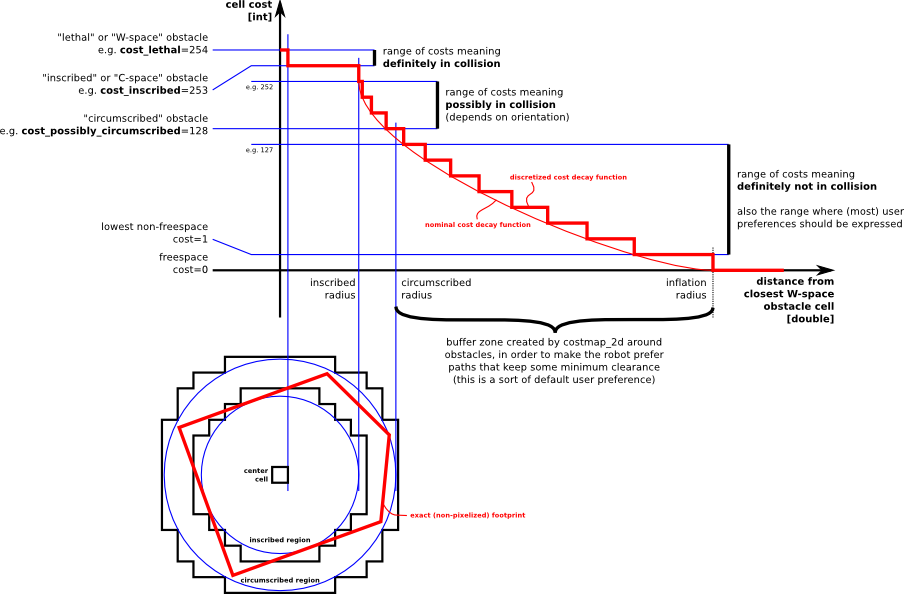
\includegraphics[width=\textwidth]{pic/costmapspec.png}
 \caption{CostMap Valuation Diagram (Source: \href{http://wiki.ros.org/costmap\_2d}{http://wiki.ros.org/costmap\_2d})}
 \label{fig:costmap}
\end{figure*}

\begin{figure*}[htbp]
 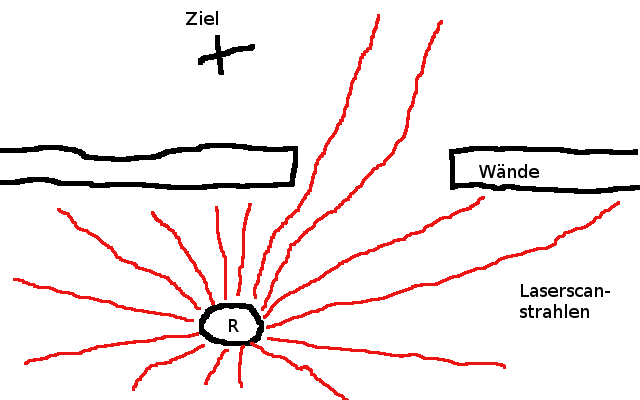
\includegraphics[width=\textwidth]{pic/simple_nav.png}
 \caption{A Simple Navigation Task}
 \label{fig:nav_task}
\end{figure*}

\section{Questions: Application Scenario}
\label{sec:questions_app_scenario}

\begin{itemize}
 \item For what is the ARTracker module?
 \item How is it possible that two TurtleBots communicate about positions, without having a common map?
 \item For what did we use the laser scanner?
\end{itemize}


